\begin{frame}{Allgemeines}{Über Arrays}
	\begin{itemize}
		\item Einfachste Listenstruktur
		\item Speichert Daten sequentiell im Speicher
		\item In der Regel nur in einer Dimension
		\item Aber auch "`mehrdimensionale"' Arrays möglich
		\item Logisch (und auch vom Zugriff) könnte man Arrays vergleichen mit:
		\begin{itemize}
			\item Vektoren bei eindimensionalen Arrays
			\item Matrizen für zwei- oder höherdimensionale Arrays
		\end{itemize}
	\end{itemize}
\end{frame}

\begin{frame}{Eigenschaften}{Von Arrays}
	\begin{itemize}
		\item Belegen einen fortlaufenden Bereich im Speicher
		\item Dadurch:
		\begin{itemize}
			\item Muss die Größe bei Initialisierung bekannt sein
			\item Sind Zugriffe auf die Elemente sehr schnell
			\item Löschen-/Einfügen von Elementen jedoch vergleichsweise "`teuer"'
		\end{itemize}
		\item Technisch ist ein Array meist lediglich ein Zeiger auf den Beginn des Arrays
		\item Arrays sind meist für Datenmengen mit vielen Elementen(Ab ~65535) ungeeignet
		\item Warum?
	\end{itemize}
\end{frame}

\begin{frame}{Datenstruktur von Arrays}{Bildlich dargestellt}
	\begin{figure}
		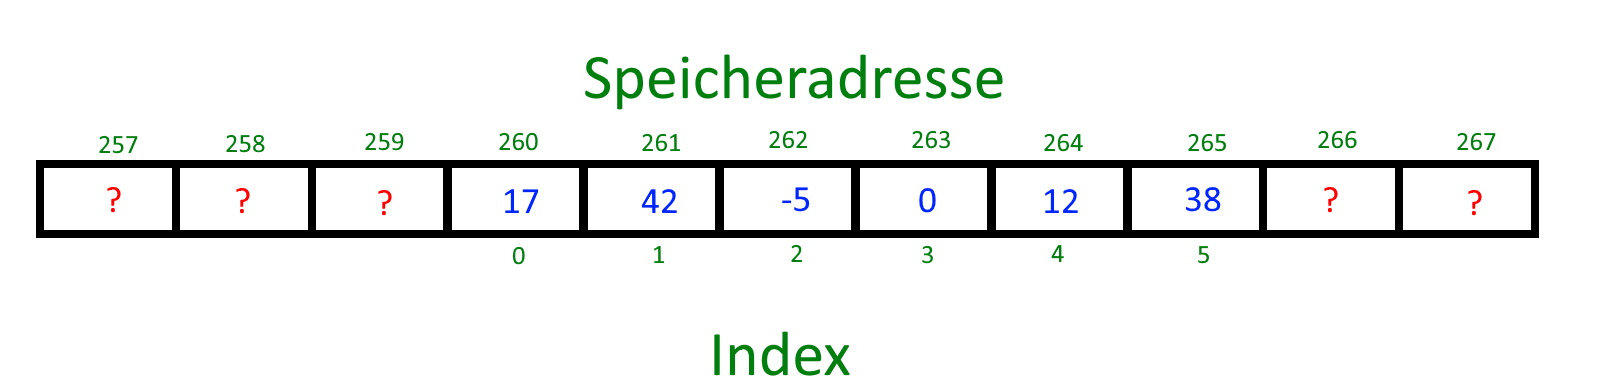
\includegraphics[width=\textwidth]{graph/Array_base}
	\end{figure}
\end{frame}

\begin{frame}{Grundoperationen}{Anlegen eines Arrays}
	\begin{itemize}
		\item Bei Anlegen eines Arrays muss immer die Größe festgelegt werden
		\item Vorher können keine Elemente hinzugefügt bzw. manipuliert werden
		\item Bei Initialisierung des Arrays wird ein Speicherbereich für dieses reserviert
		\item Größe des Speicherbereichs für ein Array der Größe $N$ ergibt sich aus:
	\end{itemize}
	$Speicher_Byte=GrößeElement_Byte\cdot N$
\end{frame}

\begin{frame}{Grundoperationen}{Zugriff auf Elemente}
	\begin{itemize}
		\item Zugriffe auf Listenelemente passieren immer in konstanter Zeit
		\item Dadurch ergibt sich die Komplexität zu: $O(1)$
		\item Begründung:
		\begin{itemize}
			\item Elemente liegen "`hintereinander"' im Speicher $\rightarrow$ Haben fortlaufende Speicheradressen
			\item Die Adresse des ersten Elements ist immer bekannt
			\item Heißt, bei Abrufen des $n$-ten Elements muss von der Startadresse nur eine bestimmte Schrittzahl addiert werden
			\item Jeder Zugriff auf ein Element ist somit (auf unterster Ebene) eine Addition und eine Leseoperation
		\end{itemize}
	\end{itemize}
\end{frame}


\begin{frame}{Graphische Darstellung}{Zugriff auf Elemente}
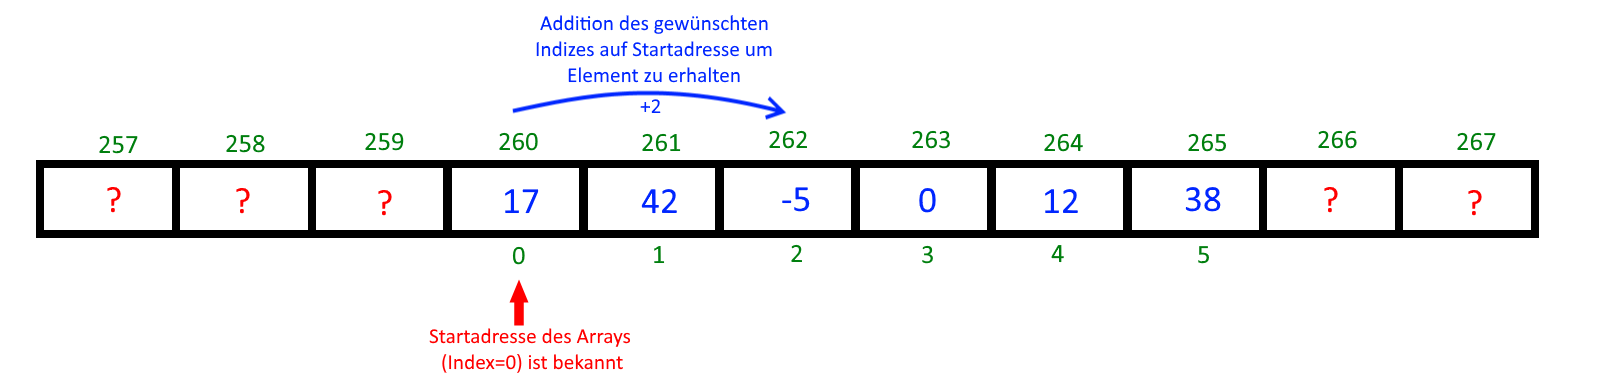
\includegraphics[width=\textwidth]{graph/array_access}
\end{frame}

\begin{frame}{Grundoperationen}{An-/Einfügen von Elementen}
	\begin{itemize}
		\item Nachträgliches Einfügen von Elementen ist nicht trivial
		\item Grund dafür ist die Speicherstruktur von Arrays
		\item Dadurch, dass die Elemente fortlaufend im Speicher liegen...
		\begin{itemize}
			\item ...müsste bei Einfügen sichergestellt sein, dass der nachfolgende Speicher noch nicht genutzt ist (Was meist nicht der Fall ist)
			\item ...und alle Elemente die nach dem eingefügten Element liegen, nach rechts "`verschoben"' werden
		\end{itemize}
		\item Dadurch häufig das anlegen eines neuen Arrays nötig
		\item Und das ausführen von vielen Kopieroperationen
	\end{itemize}
\end{frame}

\begin{frame}{Einfügen in Arrays}{Visualisiert}
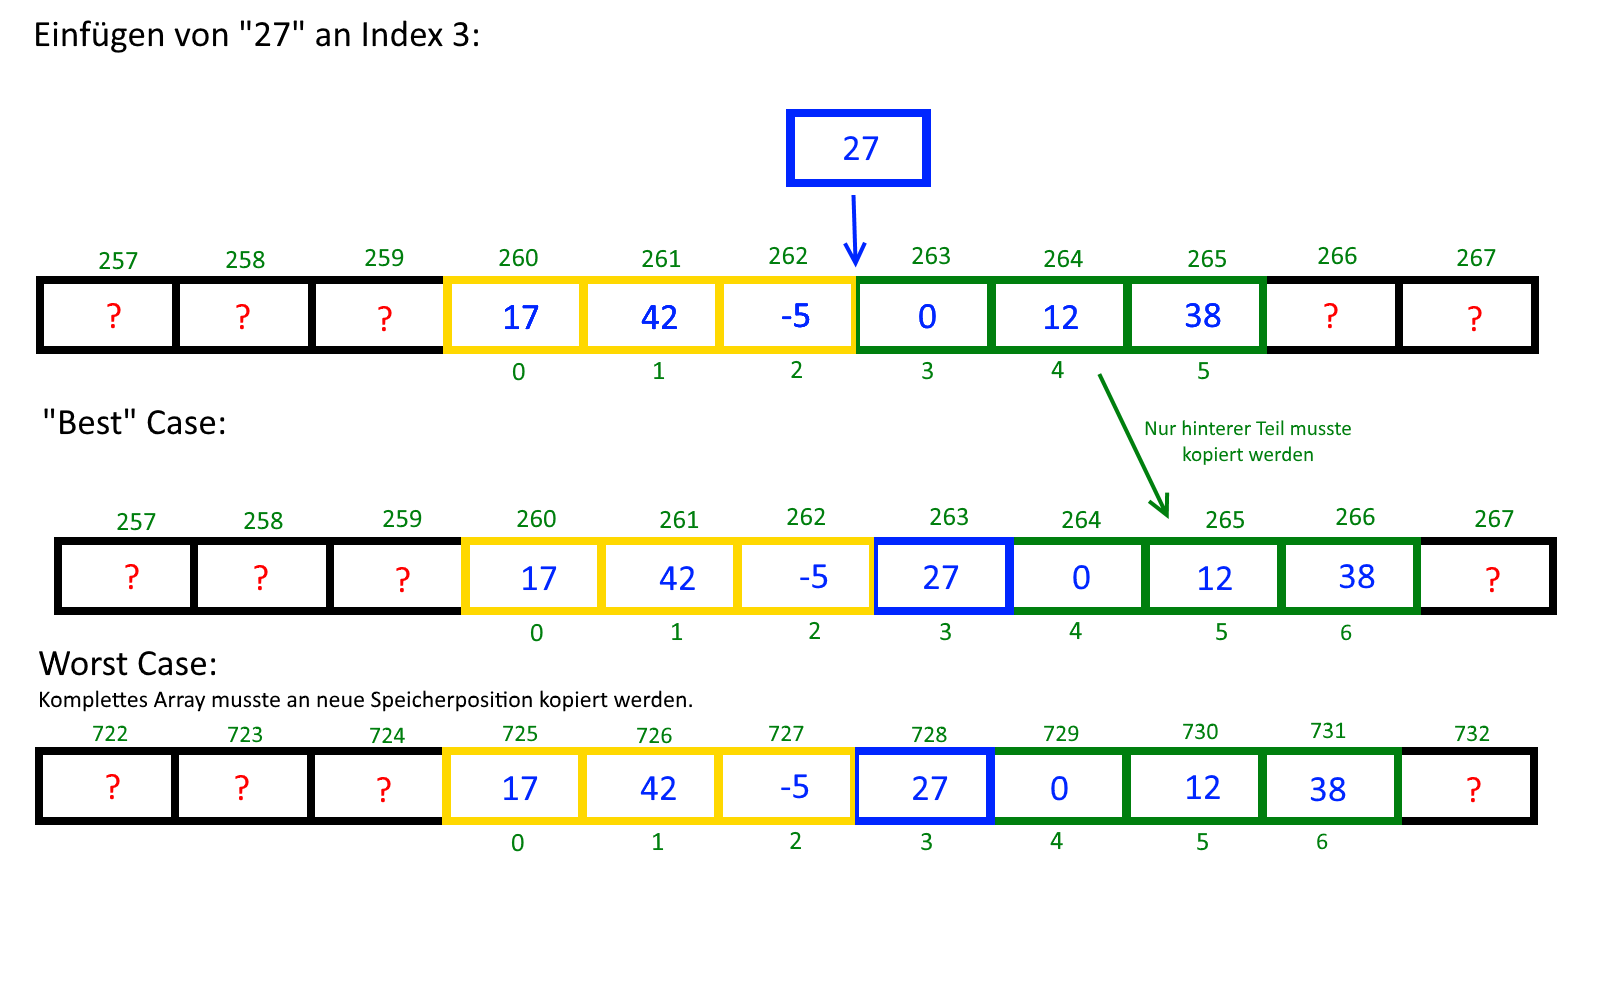
\includegraphics[height=6cm]{graph/array_insert}
\end{frame}

\begin{frame}{Komplexität}{Beim einfügen}
	\begin{itemize}
		\item Theoretischer Best-Case:
		\begin{itemize}
			\item Einfügen am Ende des Arrays
			\item ...solange der nachfolgende Speicher noch ungenutzt ist
			\item Dann wäre lediglich eine Kopieroperation erforderlich
		\end{itemize}
		\item In der Regel kann jedoch davon ausgegangen werden, dass...
		\begin{itemize}
			\item ...ein neues Array (an einem anderen Speicherbereich) angelegt werden muss
			\item ...und jedes Element des Arrays kopiert werden muss
		\end{itemize}
		\item Komplexität ergibt sich hierbei zu: $O(N)$
	\end{itemize}
\end{frame}

\begin{frame}{Ermitteln der Länge}{In Arrays}
	\begin{itemize}
		\item Bestimmen der Elemente eines Arrays nicht trivial möglich
		\item Da Array nur einen Speicherbereich beschreibt und seine eigene Größe nicht kennt
		\item Zählen von Elementen nicht möglich, da Abbruchbedingung nicht bekannt
		\item Größe muss somit selbst gespeichert und verwaltet werden
		\begin{itemize}
			\item Passiert in Java automatisch
			\item Da ein Array auch immer ein Objekt ist
			\item Bestimmen der Größe über das \texttt{length} Attribut
		\end{itemize}
	\end{itemize}
\end{frame}

\begin{frame}{Entfernen von Elementen}{In Arrays}
	\begin{itemize}
		\item Entfernen führt zu Problem im Speicherbereich:
		\item Durch das Entfernen würde eine "`Lücke"' im Array entstehen
		\item Daten im Array müssen jedoch fortlaufenden Speicher belegen
		\item D.h., Alle Elemente hinter dem entfernten Element müssen eine Position nach links verschoben werden
		\begin{itemize}
			\item "`Teure"' Kopiervorgänge nötig
		\end{itemize}
		\item Komplexität ergibt sich somit zu $O(N)$ (Worst-Case)
	\end{itemize}
\end{frame}

\begin{frame}{Entfernen von Elementen}{Visualisiert}
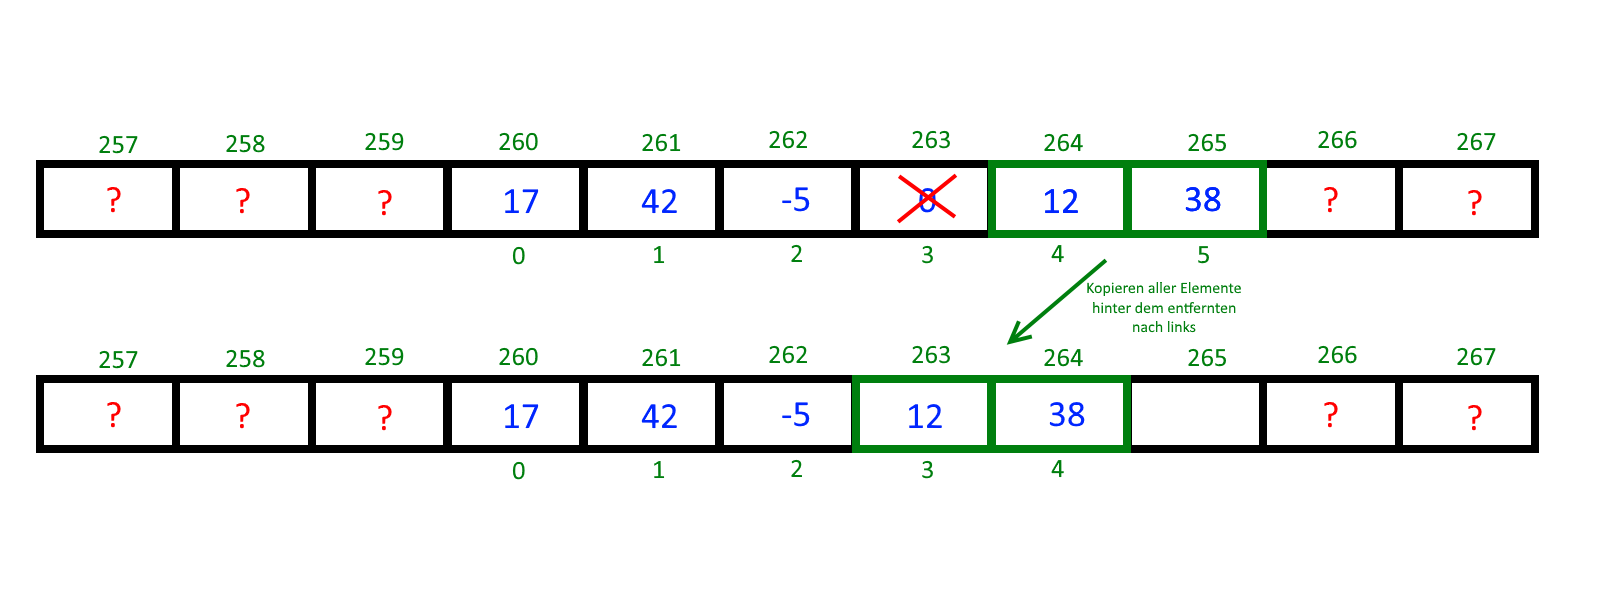
\includegraphics[width=\textwidth]{graph/array_remove}
\end{frame}

\begin{frame}{Entfernen von Elementen}{Weitere Aspekte}
	\begin{itemize}
		\item Beim entfernen von Elementen wird hinten Speicher "`frei"'
		\item Dieser ist (technisch) noch dem Array zugeordnet
		\begin{itemize}
			\item Heißt: Größe des Arrays muss theoretisch aktualisiert werden (Wenn man diese manuell verwalten muss)
		\end{itemize}
		\item Freigewordener Speicher kann jedoch später wiederverwendet werden:
		\begin{itemize}
			\item Elemente können theoretisch hinzugefügt werden ohne, dass das Array vergrößert werden muss
			\item Dafür müssen dann jedoch zwei Werte getracked werden:
			\item Die reservierte Größe des Arrays
			\item Die aktuell genutzte Größe des Arrays
			\item \texttt{ArrayList} Implementierung arbeitet ähnlich
		\end{itemize}
	\end{itemize}
\end{frame}

\begin{frame}{Konkatinieren von Arrays}
	\begin{itemize}
		\item Beim kombinieren zweier Arrays ergibt sich ähnliches Problem wie beim Einfügen
		\item Array hat ggf. nicht genug Platz um Elemente von beiden Arrays aufzunehmen
		\item Daher sind meist folgende Schritte nötig um zwei Arrays mit Länge $N$ und $M$ zu kombinieren:
		\begin{itemize}
			\item Anlegen eines neues Arrays mit Größe $N+M$
			\item Kopieren aller Elemente des ersten Arrays in den vorderen Teil
			\item Kopieren aller Elemente des zweiten Arrays in den hinteren Teil
		\end{itemize}
		\item Dadurch ergibt sich die Komplexität zu $O(N+M)$ (inklusive Overhead für Anlegen des neuen Arrays)
	\end{itemize}
\end{frame}

\begin{frame}{Vor- und Nachteile}
\end{frame}